\documentclass[a4paper, 11pt]{article} % Font size (can be 10pt, 11pt or 12pt) and paper size (remove a4paper for US letter paper)

\usepackage[T1]{fontenc}
\usepackage[utf8]{inputenc}
\usepackage[ngerman]{babel}
\usepackage{lmodern}

\usepackage[protrusion=true,expansion=true]{microtype} % Better typography
\usepackage{graphicx} % Required for including pictures
\usepackage{wrapfig} % Allows in-line images
\usepackage{amssymb,amsmath}
\usepackage{subfigure}
\usepackage{cite}
\usepackage{mathpazo} % Use the Palatino font
\linespread{1.05} % Change line spacing here, Palatino benefits from a slight increase by default

\usepackage{tikz-uml}
%\usepackage{tikz}
%\usepackage{ifthen}
%\usepackage{xstring}
%\usepackage{calc}
%\usepackage{pgfopts}

\usepackage{listings}

%\setlength\parindent{0pt}%Festlegen des Absatzeinzuges
%\setlength\mathindent{0pt}%Festlegen des Einzuges für abgesetzte Formeln

\makeatletter
\renewcommand\@biblabel[1]{\textbf{#1.}} % Change the square brackets for each bibliography item from '[1]' to '1.'
\renewcommand{\@listI}{\itemsep=0pt} % Reduce the space between items in the itemize and enumerate environments and the bibliography

\renewcommand{\maketitle}{ % Customize the title - do not edit title and author name here, see the TITLE block below
\begin{flushright} % Right align
{\LARGE\@title} % Increase the font size of the title

\vspace{50pt} % Some vertical space between the title and author name

{\large\@author} % Author name
\\\@date % Date

\vspace{40pt} % Some vertical space between the author block and abstract
\end{flushright}
}

\title{\textbf{Dokumentation gMix-Simulator GUI}\\ % Title
Benutzer- / Entwicklerhandbuch} % Subtitle

\author{\textsc{Beifuß A. ; Langnickel J. ; Lohmueller J. C. ; Weinschenk M.} % Author
\\{\textit{Universität Hamburg - MIN Falkultaet - Informatik - SVS}}} % Institution

\date{\today} % Date

\begin{document}

\maketitle % Print the title section

%\renewcommand{\abstractname}{Summary} % Uncomment to\texttt{} change the name of the abstract to something else
 
% \begin{abstract}

% \end{abstract}

\tableofcontents

% \hspace*{3,6mm}\textit{Keywords:} lorem , ipsum , dolor , sit amet , lectus % Keywords

\vspace{30pt} % Some vertical space between the abstract and first section

\section{Einleitung} % (fold)
\label{sec:einleitung}

\subsection{gMix (Todo Malte)} % (fold)
\label{sub:gmix}
Dieser Abschnitt behandelt das Thema Mixe und motiviert die Entwicklung des gMix-Simulators.
% subsection gmix (end)

\subsection{Ziele der GUI (Todo Malte)} % (fold)ssu
\label{sub:ziele_der_gui}
In diesem Abschnitt werden die unterschiedlichen Benutzergruppen vorgestellt, für die GUI gedacht ist. Es wird analysiert, welche Anforderungen und Bedürfnisse die jeweiligen Anwendergruppen haben. Entlang der gewonnenen Erkenntnissen soll dann die GUI entwickelt werden, so dass nach Möglichkeit die Anforderungen aller Gruppen zufriedengestellt werden können.
% subsection ziele_der_gui (end)

\subsection{XML vs. Annotations (Todo Alex)} % (fold)
\label{sub:xml}
In diesem Abschnitt werden wir kurz motivieren, warum wir uns entschieden haben in der GUI auf Annotations zu setzen und XML vermeiden. 

Flexibilität / Erweiterbarkeit
Ein sehr wichtiger Aspekt ist, dass das von uns angestrebte Annotations-System sehr einfach erweiterbar sein soll. Da der \emph{gMix-Simulator} pluginbasiert ist, kann es zu einem späteren Zeitpunkt (nach Projektende) notwendig sein, dass \emph{Properites} oder \emph{Plugins} beispielsweise neue Eigenschaften erhalten. Während im Falle von XML ggf. das Schema angepasst werden und muss komplexere Eingriffe in das Parsing notwendig sein können, ist der Aufwand bei der Verwendung von Annotations sehr gering. Hier genügt es die jeweiligen Annotations (beispielsweise \emph{IntSimulationProperty}), um die notwendigen Felder zu erweitern. Die zugehörigen POJOs (beispielsweise \emph{IntProp}), welche später die Informationen aus den Annotations enthalten, müssen lediglich um \emph{Getter} und \emph{Setter} erweitert werden. Die notwendigen Änderungen am Annotations-Parser (in der Klasse \emph{SimPropRegistry}) sind ebenfalls sehr einfach und beschränken sich auf das Auslesen der Annotation und das Aufrufen von \emph{Settern}.

Dezentralisierung:
Im Gegensatz zu XML werden Annotations direkt in den Plugin-Code eingebettet. Dieses bringt gleich zwei Vorteile mit sich. Zum einen werden dadurch zentrale Dateien vermieden, wodurch eine sehr lose Kopplung ermöglicht wird, wie es bei Plugin-Systemen wünschenswert ist --- Versionskonflikte von zentralen Dateien werden so vermieden, was bei Plugin-System sehr wichtig ist. Dieses wäre auch noch mit XML möglich, würde jedoch unweigerlich in einer Unmenge an XML-Dateien enden. Der zweite Vorteil ist, dass ein Pluginentwickler die Festlegung der Eigenschaften von Properties und Plugins genau dort vornimmt, wo diese auch logisch gesehen hingehören, nämlich direkt an den Properties und den Plugins. 

Ein dritter Aspekt ist, das Annotations Teil der Sprache Java sind. Dieses bedeutet für den Entwickler, dass er bei den Programmieraufgaben mehr Unterstützung durch die IDE bekommt. So wird er bei der Erweiterung von Annotations beispielsweise frühzeitig auf syntaktische Fehler aufmerksam gemacht. Bei der Verwendung von XML ist dieses nicht gegeben, da zwischen der XML-Datei und Java-Code kein syntaktischer Zusammenhang besteht. 

% subsection xml (end)

% section einleitung (end)

\subsection{Annotations} % (fold)
\label{sub:annotations}
Dieser Abschnitt beschreibt die unterschiedlichen Annotation-Typen, welche unsere GUI verwendet. Insgesamt sind es drei unterschiedliche Typen von Annoations, die in der GUI zum Einsatz kommen. Bevor die Architektur der GUI erklärt wird, ist es sinnvoll kurz über die verschiedenen Annotations zu sprechen. Dazu gehört die Annotations-Typen zu motivieren, die Unterschiede zu erklären, auf die Felder der Annotationen einzugehen.

Zuvor wollen wir jedoch eine Grafik betrachten, um den Leser mit der von uns verwendeten Bezeichnungen in Bezug auf die GUI bekannt zu machen. In Abb. 

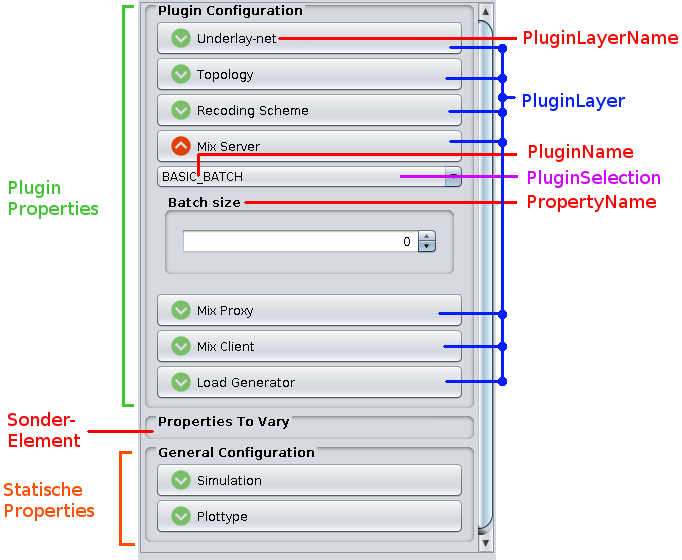
\includegraphics[scale=0.56]{img/configtool_edit.png}
% subsection annotations (end)

\begin{lstlisting}
#-OUTPUT_STRATEGY--OR--FLUSHING_ALGORITHM----------
# ...
# Some possible values: NO_DELAY, ... 
# BATCH_WITH_TIMEOUT, BINOMIAL_POOL, ... 
# COTTRELL_TIMED_POOL, DISTINCT_USER_BATCH, ... 
# DLPA_HEURISTIC_2, LOSSY_SYNCHRONOUS_BATCH, ...
# THRESHOLD_AND_TIMED_BATCH, THRESHOLD_OR_TIMED_BATCH, ... 
# TIMED_BATCH, TIMED_DYNAMIC_POOL
#	
OUTPUT_STRATEGY = BASIC_BATCH
...
BASIC_BATCH_BATCH_SIZE = 100
...
\end{lstlisting}

Hier ist 'OUTPU\_STRATEGY' der PluginLayerKey für das Plugin, welches auf der Ebene des Mix-Servers argiert. In der Experiment-Konfiguration bildet der PluginLayerKey auf ein PluginKey ab (hier 'BASIC\_BATCH') und identifiziert damit das Plugin. Das Plugin, welches den PluginKey 'BASIC\_BATCH' zugewiesen ist, hat wiederum eine Property, welche durch den PropertyKey 'BASIC\_BATCH\_BATCH\_SIZE' identifiziert wird.

Nachdem nun die grundlegenden Terminologien eingeführt wurden, ist es an der Zeit die Annotations zu betrachten, welche den Aufbau der GUI regeln. Wir gehen dabei bottom-up vor, da weniger vorweggenommen werden muss und es somit für den Leser verständlicher sein sollte.

\subsubsection{Property Annotation} % (fold)
\label{ssub:feld_annotation}
Die Property-Anotations sind wohl die wichtigsten und auch komplexesten Annotations, die wir in der GUI verwenden. Diese Annotations werden dazu verwendet um Felder im Quellcode des Simulators und im Quellcode der Plugins zu annotieren. Dabei werden solche Felder annotiert, die tatsächlich Simulation-Properties halten. Diese sind daran zu erkenne, dass ihr Wert über \emph{Simulator.settings.getProperty()}

Alle \emph{Properties} haben eine Grundmenge an Feldern, die in der folgenden Auflistung erläutert werden. Besonders sei hier \emph{BoolSimulationProperty} hervorgehoben. Dieses ist die einzige Property-Annotation, die außer dieser Grundmenge keine weiteren Felder besitzt.
\begin{itemize}
	\item name: Es handelt sich um einen String, der den Namen der Property festlegt, wie er in der GUI angezeigt werden soll. Analog zur obigen Grafik entspricht dieses dem \emph{PropertyName}.\\
	Default: keinen (Der Entwickler muss diesen Wert händisch setzen)
	\item key: Ein String der die Property innerhalb der Experiment-Konfiguration eindeutig identifiziert. Analog zum obigen Listing entspricht dieses dem \emph{PropertyKey}).
	\item value: TODO: entfernen und auf eine Default-Config umstellen!
	\item position: TODO: Muss noch implementiert werden. Dieses ist ein Integer (>= 0), der die Position des zugehörigen GUI-Elementes steuert. Je größer der Wert desto weiter unten taucht das GUI-Element der jeweiligen Proerty auf. Sollten zwei Properties eines Plugins hier den selben Wert haben, so wird lexikalisch geordnet.\\
	Defalut: 0 
	\item tooltip: Dieses ist ein String, der angezeigt wird, wenn sich die Maus über dem entsprechenden GUI-Element befindet.\\
	Default: leerer String 
	\item info: Ein String der (sofern festgelegt) als Infotext an dem entsprechenden GUI-Element der Property auftaucht.  
	Default: leerer String
	\item global: Ein Boolean über das festgelegt werden kann, dass die Property global (im gesamten PluginLayer angezeigt werden soll).\\
	Default: leerer String
	\item inject: TODO: <PluginPosition> muss wieder entfernt werden. Ein String der es erlaubt Properties an eine beliebige Stelle in der GUI zu injizieren. Dieses ist notwendig, wenn Properties beispielsweise zu einem pseudo Plugin gehören (\emph{'Recoding Scheme'} ist z.B. ein solches pseudo Plugin, das in Wirklichkeit nicht als Plugin existiert sondern viel Mehr direkt im Simulator integriert ist, dem Benutzer jedoch als Plugin dargestellt werden soll). \\
	Syntax: \"{}<LayerPosition>:<LayerKey>,<LayerName> [@<PluginPosition>:<PluginKey>,<PluginName>]\"{}\\
	Wird hier der optionale Plugin-Teil weggelassen, so gibt die Property als Layerweit (global) sichtbar.\\
	Default: false (nur im Plugin sichtbar)
	\item valueType: TODO: Entfernen! Dieser Wert sollte unter keinen Umständen von Hand gesetzt werden! 
	\item isStatic: Ein Boolean das angibt, ob eine Property im Plugin-Abschnitt (\emph{Plugin Configuration}) auftauchen soll oder aber im Abschnitt für statische Properties (\emph{General Configuration}). Dieses Feld wird nur in Kombination mit dem Feld \emph{inject} verwendet. Sinnvoll ist der Einsatz meist dort, wo es sich um Properties handelt, die nicht zu einem Plugin gehören und aus logischer Sicht auch nicht auf einer Pluginschicht liegen.\\
	Default: false (Property wird in der \emph{Plugin Configuration} angezeigt)
	\item value\_requirements: Eine Klasse, welche von der abstrakten Klasse Requirement erbt und in derer für diese Simproperty relevante Value Anforderungen umgesetzt werden.
	\item enable\_requirements: Eine Klasse, welche von der abstrakten Klasse Requirement erbt und in derer für diese Simproperty relevante Enable Anforderungen umgesetzt werden.
\end{itemize}

Die Annotations für die numerischen \emph{Properties} (\emph{IntSimulationProperty}, \emph{FloatSimulationProperty} und \emph{DoubleSimulationProperty}) haben neben den Standardfeldern  
\begin{itemize}
	\item min: Ein numerischer Wert (abhängig vom konkreten Typ der Annotation), der den Minimalwert angibt, den die Property annehmen kann. Der angegebene Wert wird von der GUI dazu verwendet um Benutzereingaben auf Gültigkeit zu prüfen.\\
	Default: Integer.MIN\_VALUE bzw. Float|Double.NEGATIVE\_INFINITY
	\item max: Ein numerischer Wert (abhängig vom konkreten Typ der Annotation), der den Maximalwert angibt, den die Property annehmen kann. Der angegebene Wert wird von der GUI dazu verwendet um Benutzereingaben auf Gültigkeit zu prüfen.\\
	Default: Integer|Float|Double.MAX\_VALUE
	\item guiElement: Ein String über den festgelegt werden kann, über was für ein GUI-Element der Wert Property in der GUI konfiguriert werden kann. Aktuell sind für Ganzzahl und Gleitkomma zahlen die beiden Elemente JSpinner (\emph{\"{}spinner\"{}} für Integer, Float und Double) und JSlider (\emph{\"{}slider\"{}} für Integer) implementiert. Beide Elemente verwenden die durch die Felder \emph{min} und \emph{max} festgelegten Grenzen und schützen den Benutzer vor Fehleingaben.\\
	Default: \emph{\"{}spinner\"{}} (JSpinner)
	\item stepSize: Ein numerischer Wert (abhängig vom konkreten Typ der Annotation), der die Schrittweite eines JSpinners angibt. Dieses Feld ist in Kombination mit \emph{guiElement=\"{}spinner\"{}} sinnvoll um die Schrittweite manuell festzulegen. So ist es bei einigen Properties vlt. besser eine Schrittweite von 0.1 zu haben, während zu anderen Properties vielleicht kleinere Schrittweiten wie 0.001 besser passen.\\
	Default: Integer 1, Gleitkomma 0.001f
	\item enableAuto: Ein Boolean über das festgelegt werden kann, dass die eigentlich numerische Property den String \"{}AUTO\"{} annehmen kann. Der Simulator sieht dieses für einige Properties vor. Im Falle, dass eine numerische Property den Wert \"{}AUTO\"{} hat, wird aus der tatsächliche Wert automatisch anhand von anderen Properties bestimmt. Wird dieses Feld auf true gesetzt, so gibt es im entsprechenden GUI-Element eine Checkbox, über die der Benutzer festlegen kann, dass die Property automatisch bestimmt werden soll. Für denn Fall, dass  die Checkbox aktiviert ist, wird das eigentliche Eingabeelement (siehe \emph{guiElement}) ausgegraut.\\
	Beispiele: Request und Reply Size in ParetoClient, PoissonClient, RequestReplyClient und SendConstantClient\\
	Default: false (keine Checkbox für \"{}AUTO\"{}) 
	\item enableUnlimited: Ein Boolean über das festgelegt werden kann, dass die eigentlich numerische Property den String \"{}UNLIMMITED\"{} annehmen kann. Dieses funktioniert analog zu \emph{enableAuto}.\\
	Beispiel: DelayBox alle sechs Bandwidth-Properties
	Default: false (keine Checkbox für \"{}UNLIMITED\"{})
\end{itemize}

Die Annotation \emph{StringSimulationProperty} hat (wie auch die numerischen \emph{Properties}) zusätzliche Felder.
\begin{itemize}
	\item possibleValues: Ein String über den vordefinierte Werte festgelegt werden können. Die einzelnen Werte werden innerhalb des Strings durch Kommata separiert. Ist dieser String ungleich dem leeren String, so wird die GUI dem Benutzer eine JCombobox zur Manipulation des Property-Wertes anbieten (es sei denn, dass \emph{multiSelection=true} ist, siehe nächstes Feld).\\
	Default: leerer String
	\item multiSelection: TODO: Implementieren. Ein Boolean über den festgelegt werden kann, dass eine Mehrfachauswahl der vordefinierten Werte möglich ist. Ist dieses Feld auf true gesetzt und sind mittels \emph{possibleValues} mehrere vordefinierte Werte angegeben, so wird ein auf einer JList basierendes GUI-Element erstellt, um eine Mehrfachauswahl zu erlauben.\\
	Default: false (Mehrfachauswahl ist deaktiviert) 
	\item regex: TODO: Implementieren! Ein String der eine Regex darstellt, die dazu verwendet wird, um Benutzereingaben auf Gültigkeit zu prüfen (kann dann ggf. auch in den ValueRequirements verwendet werden!)
\end{itemize}


% subsubsection feld_annotation (end)

\subsubsection{Plugin Annotation} % (fold)
\label{ssub:plugin_annotation}
Neben den \emph{Property Annotations} gibt es zwei weitere Typen von Annotations. Hierzu gehören unter anderem die \emph{Plugin Annotations}. Die Einführung dieser Annotations erschien uns aus dem Grund sinnvoll, da es für einen Pluginentwickler vorteilhaft ist, wenn dieser Eigenschaften die logisch gesehen zu einem Plugin gehören auch direkt am Plugin setzten kann. Ein Beispiel hierfür sind der Pluginname, der in der GUI auftaucht (z.B. ''Basic delay box'') oder aber der Schlüssel, unter dem das Plugin in der Experiment-Konfiguration auftaucht (z.B. ''BASIC\_DELAY\_BOX''). Des weiteren erlaubt eine Annotation auf Pluginebene das pluginweite setzen von Eigenschaften. So kann beispielsweise über eine \emph{Property Annotation} festgelegt werden, dass alle Properties, welche in einem Plugin liegen global sind, wodurch sich der Pluginentwickler ggf. ein wenig Schreibarbeit sparen kann. \emph{Property Annotations} haben folgende Felder:

\begin{itemize}
	\item pluginName: TODO: Muss noch implementiert werden!
	Ein String, der den Namen festlegt, unter dem das Plugin in der GUI auftritt. Entspricht der bereitgestellt String dem leeren String, so wird stattdessen \emph{pluginKey} als angezeigter Name in der GUI verwendet.\\
	Default: Der leere String
	\item pluginKey:
	Ein String, der dem Namen festlegt, unter dem das Plugin in der Experiment-Konfiguration auftritt. Dieser String muss dabei genau dem String entsprechen, der das Plugin gegenüber dem den \emph{gMix-Simulator} identifiziert (siehe Enums in \emph{evaluation.simulator.pluginRegistry}).
	Default: kein
	\item pluginLayerKey:
	Ein String, der den Layer (die Kategorie) festlegt, unter dessen Pluginauswahl das Plugin auftauchen soll. Dieses Feld ist dafür gedacht, dass der Entwickler von Hand festlegen kann, in welchem Layer das Plugin aufgelistet wird. Dieses ist notwendig, wenn ein Plugin aus mehreren Klassen besteht die keine gemeinsame Oberklasse haben. Ein Beispiel Für die Anwendung dieses Feldes ist in der Klasse \emph{StopAndGoMessage} zu finden. Dort wird mittels dieses Feld mitgeteilt, dass dieses Plugin in den Layer \"{}OUTPUT\_STRATEGY" gehört. Der Layer selbst wird aber durch die \emph{Plugin Superclass Annotation} in \emph{OutputStrategyImpl} erstellt, welches eine Oberklasse von \emph{StopAndGo} ist. ACHTUNG: Hier dürfen tatsächlich nur Keys eingetragen werden, die auch in einer \emph{Plugin Superclass Annotation} festgelegt wurden. Anderenfalls kommt es zu Fehlern!\\
	Default: leerer Sting (autodetection via \emph{Plugin Superclass})
	\item documentationURL:
	Ein String der den Pfad/Dateiname zu der Dokumentation des Plugins. Sofern hier ein Wert angegeben wird (und die referenzierte Datei existiert), wird die Dokumentation in den \emph{Help View} mit aufgenommen.\\
	Default: leerer Sting (keine Dokumentation verfügbar)
	\item visible:
	Ein boolean über das festgelegt werden kann, ob das Plugin in der Pluginauswahl auftaucht oder nicht\\
	Default: true (sichtbar)
	\item global:
	Ein boolean über das alle Properties, die zu dem Plugin gehören gobal gesetzt werden können. Global bedeutet eine Property taucht für jede Pluginwahl in der GUI auf.\\
	Default: false (nicht global)
	\item allowGlobalFields:
	Ein boolean über das festgelegt wird, ob Properties aus des Plugins global sein dürfen. Global bedeutet eine Property taucht für jede Pluginwahl in der GUI auf.\\
	Default: true (globale Properties sind erlaubt)
\end{itemize}
% subsection plugin_annotation (end)

\subsubsection{Plugin Superclass Annotation} % (fold)
\label{ssub:plugin_annotation}
Eine weitere Klasse von Annotations sind die \emph{Plugin Superclass Annoations}. 
Mit dieser Annotation werden die Oberklassen von Plugins versehen (z.B. DelayBoxImpl, ClientSendStyleImpl usw. ). Alle Properties die in einer solchen Oberklasse deklariert sind, werden als globale Properties aufgefasst und werden daher unabhängig von der im Layer getroffenen Pluginauswahl in der GUI dargestellt. 
% subsection plugin_annotation (end)

\begin{itemize}
	\item layerKey:
	Ein String der den Schlüssel festlegt, unter dem der \emph{pluginKey} des aktiven Plugins in der Experiment-Konfiguration geschrieben wird. Die aktuell verwendeten \emph{LayerKeys} der Plugins sind: 
	\begin{itemize}
		\item CLIENT\_SEND\_STYLE
		\item TYPE\_OF\_DELAY\_BOX
		\item MIX\_SEND\_STYLE
		\item OUTPUT\_STRATEGY
		\item TOPOLOGY\_SCRIPT 
		\item TYPE\_OF\_TRAFFIC\_GENERATOR
	\end{itemize}
	Default: kein (muss händisch vom Pluginentwickler gesetzt werden)
	\item layerName:
	Ein String der den Namen des Layers festlegt, welcher in der GUI angezeigt werden soll.\\
	Default: kein
	\item fakePlugins:
	Ein String der es erlaubt eine Pluginauswahl zu erstellen, für Pugins die real garnicht existieren. Diese Technik kommt beispielsweise bei \emph{TopologyScript} zum Eisatz. Die Plugins  
	\begin{itemize} 
		\item NO\_MIXES,ONE\_MIX
		\item THREE\_MIX\_CASCADE 
		\item FIVE\_MIX\_CASCADE 
	\end{itemize}
	existieren in Wirklichkeit garnicht. Sie sind lediglich Namen von Enums, die auf die auf Instanzen der echten Plugins \emph{NoMixTopology} und \emph{NMixCascadeTopology} in verschiedenen Konfigurationen abbilden. Es ist jedoch nicht gewünscht, dass der Endanwender die tatsächlichen Plugins verwendet sondern auf die vordefinierten Konfigurationen zurückgreift. \emph{fakePlugins} kann daher ein String zugewiesen werden, der eine Menge von pseudo Plugins darstellt (die Namen der pseudo Plugins werden innerhalb des Strings durch Kommata separiert, siehe \emph{TopologyScript}). Diese pseudo Plugins werden dann in die Pluginauswahl injiziert und können dort durch den Benutzer anschließend ausgewählt werden.\\
	Default: leerer String (keine gefakten Plugins in der Pluginauswahl verfügbar)
	\item position:
	Ein Integer (größer als 0) über den angegeben werden kann an welcher Position der Pluginlayer in der GUI auftaucht. Je kleiner der angegebene Wert ist, desto weiter oben wird der Pluginlayer in der GUI angezeigt. Haben zwei unterschiedliche Pluginlayer den selben Wert bei der Position, so wird lexikalisch sortiert.\\
	Default: 100 
\end{itemize}

\section{Architektur} % (fold)
\label{sec:architektur}
In diesem Abschnitt wird die Architektur der \emph{gMix-Simulator-GUI} erklärt und das Zusammenspiel der einzelnen Komponenten ausführlich erläutert. 

\subsection{Übersicht der Architektur} % (fold)
\label{ssub:uebersicht}

TODO: Muss auf einen neuen Stand gebracht werden!!!

\begin{figure}[!htp]
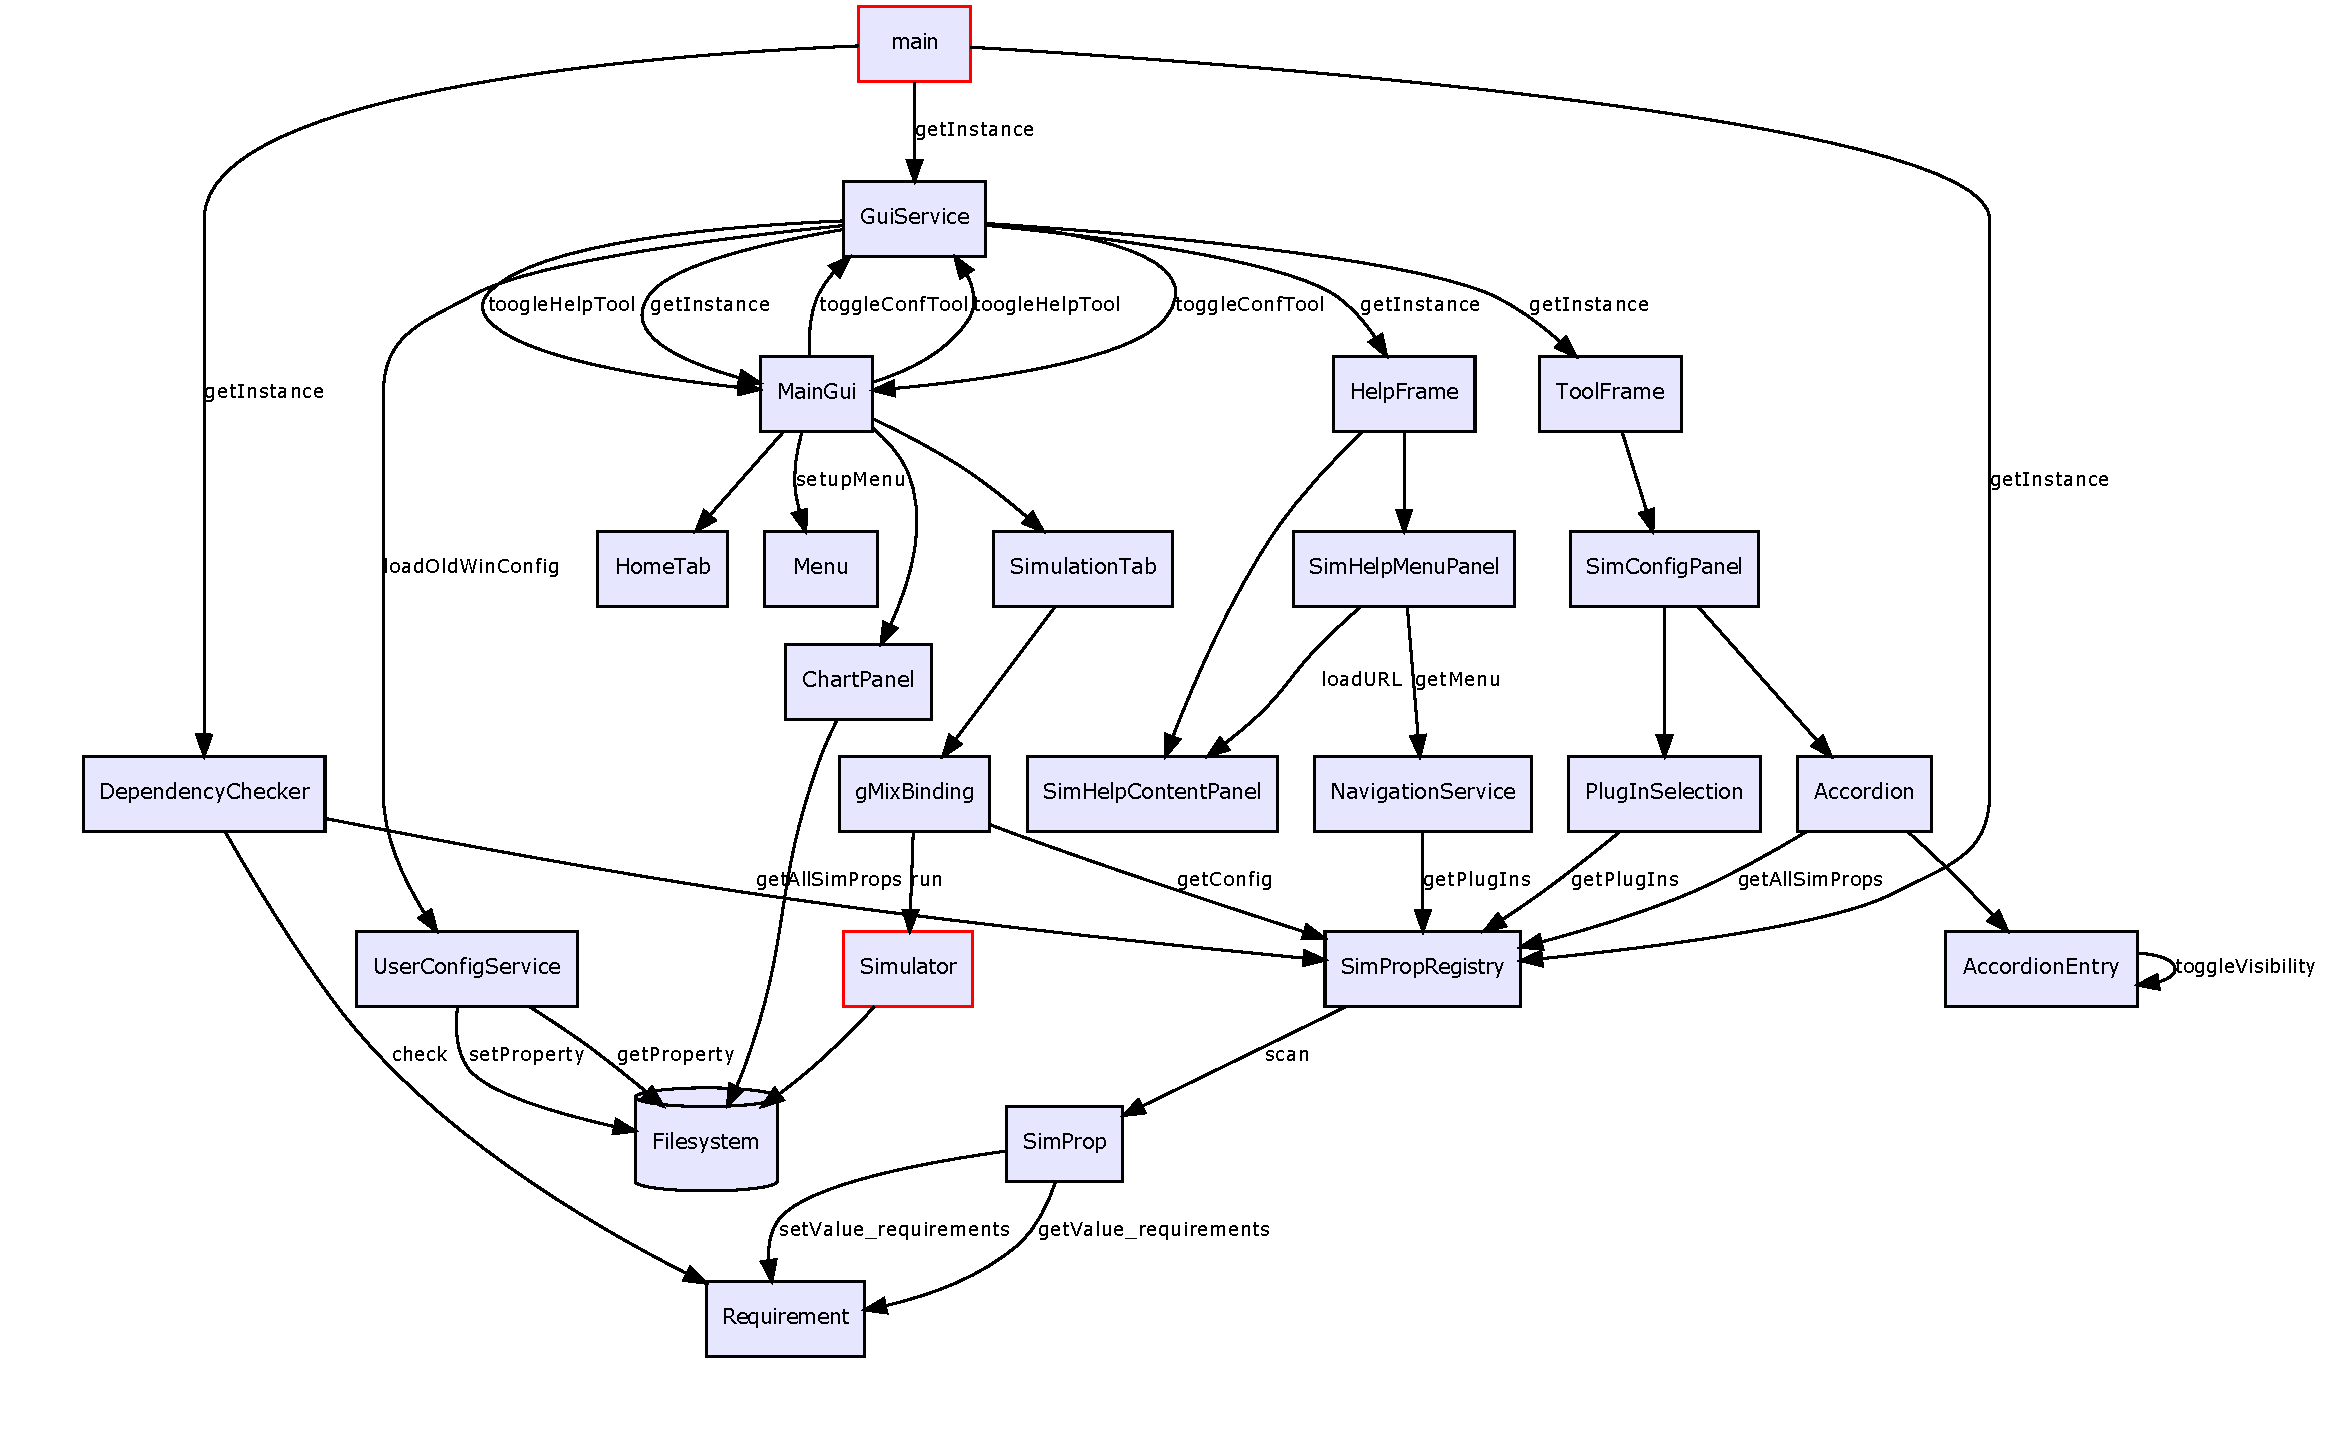
\includegraphics[width=\textwidth]{dot/arch}
\caption{Aufrufhierarchie}
\label{fig:callgraph}
\end{figure}

% subsubsection uebersicht (end)

\subsection{Einzelne Komponenten} % (fold)
\label{ssub:einzelne_komponenten}
In diesem Unterabschnitt werden die wichtigsten Komponenten der \emph{gMix-Simulator-GUI} behandelt.

\subsubsection{SimPropRegistry}
\label{sssub:simpropregistry}
Die Klasse \emph{SimPropRegistry} ist die wichtigste Hauptkomponenten der gMix-Simulator-GUI. Ihre Aufgabe besteht darin, den gesamten Code des gMix-Simulators nach Annotations abzusuchen und die in den Annotations enthaltenen Informationen zu verarbeiten. Die \emph{SimPropRegistry} kennt dabei drei unterschiedliche Typen von Annotationen.

\begin{enumerate}
	\item Property Annotations (aka. SimProp)
	\item Plugin Annotations (aka. SimGuiPlugin)
	\item PluginSuperclass Annotations (aka. SimGuiPluginSuperclass)
\end{enumerate}

Die einzelnen Annotation-Typen wurden in Abschnitt \ref{sub:annotations} erläutert. Die \emph{SimPropRegistry} erzeugt anhand dieser Annotations dann Plugin- und Property-Objekte, welche zur Laufzeit in verschiedenen Maps verwaltet werden. Neben den beiden wichtigsten Maps (\emph{properties} und \emph{plugins}), werden noch weitere Maps gehalten, welche beispielsweise die Menge der aktuell in der GUI ausgewählten Plugins halten (\emph{activePlugins}) oder ...

Des weiteren bietet die \emph{SimPropRegistry} einige Methoden an, um auf die Inhalte eben dieser Maps zuzugreifen. So beispielsweise eine Methode (\emph{setValue}), um Werte einer vorhandenen Property zu ändern. Die Plugin-Objekte hingegen sind komplett unveränderlich, da sie keine Informationen halten, die vom Benutzer editierbar sind --- zur Zeit enthält ein Plugin-Objekt lediglich die Information, wo die zugehörige Dokumentation zu finden ist. Es gibt allerdings die Methode (\emph{setActivePlugins}. Mit ihr kann die Auswahl der aktiven Plugins festgelegt werden. Die Information darüber welche Plugins aktiv sind, muss der \emph{SimPropRegistry} bekannt sein, da dieses beim Schreiben der Konfiguration wichtig ist. Wir haben uns entschieden diese Informationen direkt in der \emph{SimPropRegistry} zu halten. Bei einer Zustandsänderung wird dann die \emph{SimPropRegistry} informiert. Alternativ wäre es auch möglich gewesen, dass die \emph{SimPropRegistry} an kritischen Stellen das entsprechende GUI-Element nach seinem aktuellen Zustand fragt, dieses würde jedoch eine höhere Kopplung bedeuten, da die \emph{SimPropRegistry} dann die relevanten GUI-Elemente kennen müsste.

Die \emph{SimPropRegistry} selbst ist als Singleton implementiert. Der Zugriff auf die \emph{SimPropRegistry} erfolgt über eine statische Methode (\emph{getInstance}) und kann an jeder Stelle im Code durchgeführt werden --- Diese Entscheidung wurde getroffen, da dieser Dienst in sehr vielen Komponenten der GUI verwendet wird und ein Durchreichen der Referenz in alle Komponenten sehr aufwändig und unübersichtlich wäre. 

\subsubsection{SimProp} % (fold)
\label{ssub:simprop}
Die Klasse \emph{SimProp} ist eine abstrakte Klasse und bildet die Oberklasse für die fünf typabhängigen Unterklassen (siehe Abb. \ref{fig:field_annotation}), die es zur Laufzeit geben kann.

\begin{figure}[!htp]
\begin{tikzpicture}
\umlsimpleclass[fill=blue!10]{SimProp}
\umlemptyclass[x=-3.5, y=-2, fill=blue!10]{BoolProp}
\umlemptyclass[x=-1.2, y=-2, fill=blue!10]{IntProp}
\umlemptyclass[x=1.2, y=-2, fill=blue!10]{FloatProp}
\umlemptyclass[x=3.9, y=-2, fill=blue!10]{DoubleProp}
\umlemptyclass[x=6.7, y=-2, fill=blue!10]{StringProp}
\umlVHVinherit[arm2=-1.2cm]{BoolProp}{SimProp}
\umlVHVinherit[arm2=-1.2cm]{IntProp}{SimProp}
\umlVHVinherit[arm2=-1.2cm]{FloatProp}{SimProp}
\umlVHVinherit[arm2=-1.2cm]{DoubleProp}{SimProp}
\umlVHVinherit[arm2=-1.2cm]{StringProp}{SimProp}
\end{tikzpicture}
\caption{Vererbung der Property Annotations}
\label{fig:field_annotation}
\end{figure}

 Obwohl alle Typen sehr viele Gemeinsamkeiten aufweisen, ist eine Typunterscheidung notwendig, da je nach Typ sich die Annotations ein klein wenig unterscheiden (siehe \ref{ssub:feld_annotation}). So ergibt es beispielsweise keinen Sinn, einem \emph{boolean} oder \emph{String} einen Minimal- oder Maximalwert zuweisen zu wollen, während dieses bei \emph{int}, \emph{float} und \emph{double} durchaus sinnvoll erscheint. Ein weiterer Vorteil ist, dass die Typkonversion und die Prüfung auf gültige Eingaben (sowie die Fehlerbehandlung) auch in die Unterklassen ausgelagert werden können, was der Lesbarkeit des Codes sehr dienlich ist. 

\subsubsection{SimGuiPlugin} % (fold)
\label{ssub:simprop}
Der Zweck der Klasse \emph{SimGuiPlugin} besteht darin, statische Informationen bezüglich eines Plugins zu halten, wie beispielsweise den Pfad zu der Plugin-Dokumentation. Diese Information kann nämlich vom \emph{Help View} abgefragt werden, so dass dort ein entsprechend verlinkter Eintrag auftaucht.  

Weiterhin ist eine Funktionalität in \emph{SimGuiPlugin} ausgelagert, welche es erlaubt als \emph{PluginSuperClass} annotierte Oberklassen ausfindig zu machen. 

\subsubsection{GUI-Elemente}
\label{sssub:guiservice}
TODO: Jan

\textbf{Configuration View} % (fold)
\label{ssub:accordion}

\textbf{Simulation View} % (fold)
\label{ssub:accordion}

\textbf{Result View} % (fold)
\label{ssub:accordion}

\textbf{Help View} % (fold)
\label{ssub:accordion}

\textbf{Konsole} % (fold)
\label{ssub:accordion}

\subsubsection{UserConfigService} % (fold)
\label{ssub:userconfigservice}
Der UserConfigService verwaltet die user.properties. In dieser Datei werden benutzerspezifische Einstellungen abgespeichert. Der Zugriff auf diese Datei ist nur aus dieser Klasse möglich. Beispiele für benutzerspezische Einstellungen sind z.B. die größe der einzelnen Fenster und ob sie separiert dargestellt werden.

\subsubsection{Requirement} % (fold)
\label{ssub:requirement}
Um die Abhängigkeiten zwischen verschiedenen Propertys darzustellen werden Requirements (Anforderungen) verwendet. Eine Anforderung wird dabei immer speziell für eine Property geschrieben. Um dem Entwickler maximale Freiheit zu gewähren kann die Abhängigkeit beliebig komplex gewählt werden.
Generell wird zwischen zwei Anforderungen unterschieden:
\begin{enumerate}
	\item Enable Requirements: Anforderungen die dazu führen das bestimmte Propertys in Abhängigkeit zu anderen Property und deren Werten aktiviert oder deaktiviert werden.
	\\Ein Beispiel hierfür ist das "`Simulation Time End"' Requirement. Die Simulation kann entweder durch "`Real Time"' beendet werden oder durch "`Simulation Time"'. Die beiden Optionen schließen sich somit gegenseitig aus. Daher ist es hier sinnvoll sie entsprechend zu deaktivieren/ aktivieren um den Benutzer zu unterstützen.
	\item Value Requirements: Anforderungen die dazu führen das bestimmte Propertys in ihrem Wertebereich eingeschränkt werden. Dabei wurde die Implementation so gewählt, dass der vom Plugin Entwickler gewählte Wertebereich nicht erweitert werden kann weil dieses zu nicht sinnvollen Ergebnissen im Simulator führen würde.
	\\ Ein Beispiel für ein Value Requirement ist die Einschränkung aufgrund von Minimal und Maximalwerten. Wenn eine Abhängigkeit zwischen diesen festgelegt wurden gilt u.a. das aktuelle Maximalwert nicht kleiner sein darf als der aktuelle Minimalwert.
\end{enumerate}


\subsubsection{DependencyChecker}
\label{sssub:dependencychecker}
Der Dependency Checker dient der Überprüfung von verschiedenen Abhängigkeiten von einzelnen in den SimProperties definierten Anforderungen (Requirements).
Der check findet bei jeder Änderung in der GUI statt. Im Fehlerfall, also wenn eine Anforderungen nicht eingehalten wird, gibt es zwei Fehlermechanismen:
\begin{enumerate}
	\item Enable Requirements: Die momentan nicht mögliche Simproperty wird deaktiviert. Somit ist ein Auswählen / ändern nicht mehr möglich.
	\item Value Requirements: Falls neu gesetzte Werte aufgrund von Abhängigkeiten nicht mehr möglich sind werden individuelle, in den Value Requirements definierte, Fehlermeldungen direkt in der Simpropery angezeigt.
\end{enumerate}

% subsubsection accordion (end)

\subsubsection{gMixBinding} % (fold)
\label{ssub:gmixbinding}
Die Klasse \emph{gMixBinding} ist eine Helfer-Klasse, die von der GUI verwendet wird, um dem \emph{gMix-Simulator} mit der Konfiguration aus der GUI aufzurufen. Dazu war es notwendig, den Konstruktor des \emph{gMix-Simulators} so zu erweitern, dass er die Konfiguration als \emph{passthroughParameters} entgegennimmt. Der Aufruf des Simulators erfolgt als neuer Thread. Damit blockiert die GUI nicht, während die Simulation durchgeführt wird. Nachdem der Aufruf des \emph{gMix-Simulators} zurückkehrt, wird der Pfad zum Plot an eine Factory weitergereicht, welche ein GUI-Element (\emph{}) erstellt, das für die Darstellung der Ergebnisse verantwortlich ist.

Ein bislang ungenutztes Feature, welches aber berücksichtigt wurde ist, dass in dem \emph{gMixBinding} das \emph{ResultSet} bereitgestellt wird des Simulators. Dieses beinhaltet die während der Simulation aufgezeichneten Statistik und kann dazu verwendet werden Ergebnisse in einer anderen Weise zu plotten, als es in der Konfiguration steht --- dieses Feature ist allerdings noch Zukunftsmusik. 

\section{Features} % (fold)
\label{sec:features}
Hier sollen später die Features unserer GUI aufgelistet und erklärt werden!

TEST \cite{dummy:svs}.
% section features (end)

\bibliographystyle{plain}

\bibliography{references}

%----------------------------------------------------------------------------------------

\end{document}